\let\RaggedRight\raggedright
\let\raggedright\relax
\documentclass[utf8,9pt,mathserif,usepdftitle=false]{beamer}

\usepackage{graphicx}%
\usepackage{float}%
\usepackage{wrapfig}%

\let\RaggedRight\raggedright
\let\raggedright\relax
\documentclass[utf8,9pt,mathserif,usepdftitle=false]{beamer}

\usepackage{graphicx}%
\usepackage{float}%
\usepackage{wrapfig}%

\let\RaggedRight\raggedright
\let\raggedright\relax
\documentclass[utf8,9pt,mathserif,usepdftitle=false]{beamer}

\usepackage{graphicx}%
\usepackage{float}%
\usepackage{wrapfig}%

\let\RaggedRight\raggedright
\let\raggedright\relax
\documentclass[utf8,9pt,mathserif,usepdftitle=false]{beamer}

\usepackage{graphicx}%
\usepackage{float}%
\usepackage{wrapfig}%

\include{present.daf}

% \setbeameroption{show notes on second screen}
\setbeameroption{hide notes}
\mode<presentation>
{
  \usetheme{default}
  %\usecolortheme{default} % dove, beaver
  \usecolortheme{whale}
  %\usefonttheme{serif}
}

\hypersetup{%
  pdfinfo={%
    Title={Защита курсовых работ, ИГУ},%
    Subject={О воспроизводимости результатов численных решений уравнения осцилляции нейтрино в среде},%
    Author={Данеко Илья},%
    Keywords={neutrino oscillation in matter;quality properties}%
  }
}

\title{Качественные свойства решений уравнения осцилляций нейтрино в среде
}%
\author{Данеко И.И.}
\date[ИГУ, 2025]{%
  20 октября 2025\\%
  \vspace*{10ex}%
  \begin{flushright}
    \small
    Научный руководитель: Ломов В.П.\par
  \end{flushright}
  {\vspace*{7ex}
    \footnotesize%
    Иркутск, ФГБОУ ВО ИГУ\par%
  } }

\begin{document}

\begin{frame}
  \titlepage
\end{frame}

\begin{frame}
  \frametitle{Введение}%
  %%%
  % TODO:
  \begin{itemize}
  \item<1->
   Нейтрино — одна из самых необычных частиц в нашем мире.
   
   \item<2->
   Она обладает нулевым зарядом, полуцелым спином и участвует только в слабом
   взаимодействии.
  
  \item<3-> 
  Нейтрино существует как бы в двух видах: флейворные нейтрино и
  массивные. Первые рождаются, тогда как вторые — распространяются.
 
  
  \item<4->% 
   В данной работе мы разбираем качественные
  характеристики численного решения уравнения осцилляции нейтрино в среде.
  \end{itemize}
\end{frame}

\begin{frame}
  \frametitle{Осцилляции нейтрино}%
  %%%
  Три известных состояния флейворных  \({\nu_{\alpha}}(\alpha= e, \mu, \tau)\) являются линейными комбинациями состояний массивных \({\nu_{i}}\) c массами \(m_{i}(i=1,2,3)\), состояния флейворных нейтрино являются суперпозицией состояний массивные нейтрино
  
  \onslide<2->%
  \begin{equation*}\label{eq:1}
  	{\nu_{\alpha}}=\sum_{i}U_{\alpha i}^{*}{\nu_{i}},
  \end{equation*} 
  \(U_{\alpha i}\) являются элементами унитарной матрицы
  смешивания и называемой матрицей Понтекорва–Маки–Накагавы–Сакаты (PMNS).
  
  \onslide<3->%
  Вероятность иметь состояние аромата \(\beta\) в точке r
  \begin{equation*}
  	P_{\alpha\beta}=\sum_{j}|U_{\beta j}|^{2}|A_{j}|^{2}+2\sum_{i>j}Re[U_{\beta i}U_{\beta j}^{*}A_{i}A_{j}^{*}\exp^{-\imath\Delta_{ij}L}].
  \end{equation*}
  Здесь \(\Delta_{ij}=\Delta m_{ij}^2/2E\), где \(E=|p|\), а \(A_{i}\) амплитуда вероятности наличия в точке регестрации
\end{frame}

\begin{frame}
  \frametitle{Осцилляции нейтрино в веществе}%
  %%%
  Уравнение осцилляций в среде
  \begin{equation*}
  	\imath \frac{\partial \Psi}{\partial \xi}=H(\xi)\Psi(\xi).\quad
  \end{equation*}
   \onslide<2->%
  Здесь \({H(\xi)}\) — эрмиртовая матрица
  \begin{equation*}
  	H(\xi)=H_0+\upsilon(\xi)W
  \end{equation*}
   \onslide<3->%
  Матрица \(W\) имеет вид:
  \begin{equation*}
  	W=
  	\begin{pmatrix}
  		c_{13}^{2}c_{12}^{2} & c_{12}s_{12}c_{13}^{2} & c_{12}c_{13}s_{13}\\
  		c_{12}s_{12}c_{13}^{2} & s_{12}^{2}c_{13}^{2} & s_{12}c_{13}s_{13}\\
  		c_{12}s_{13}c_{13} & s_{12}c_{13}s_{13} & s_{13}^{2}
  	\end{pmatrix}.
  \end{equation*}

  \onslide<4->%
  Профиль плотности для солнечной модели
  
  \begin{equation*}
  	\upsilon(\xi)=\gamma exp(-\eta\xi)
  \end{equation*}
  

\end{frame}

\begin{frame}
  \frametitle{Наблюдаемые}%
  %%%
  Вероятность иметь состояние аромата \(\beta\) в точке r
  \begin{equation*}
  	P_{\alpha\beta}=\sum_{j}|U_{\beta j}|^{2}|A_{j}|^{2}+2\sum_{i>j}Re[U_{\beta i}U_{\beta j}^{*}A_{i}A_{j}^{*}\exp(-\imath\Delta_{ij}L)].
  \end{equation*}
  
  \onslide<2->%
  средняя вероятность выживания составляет
  \begin{equation}
  	\langle P_{ee} \rangle=c_{12}^{2}c_{13}^{2}|\Psi_{1}|^{2}+s_{12}^{2}c_{13}^{2}|\Psi_{2}|^{2}+s_{13}^{2}|\Psi_{3}|^{2}.
  \end{equation}
\end{frame}

\begin{frame}
	\frametitle{Качественные свойства решения}%
	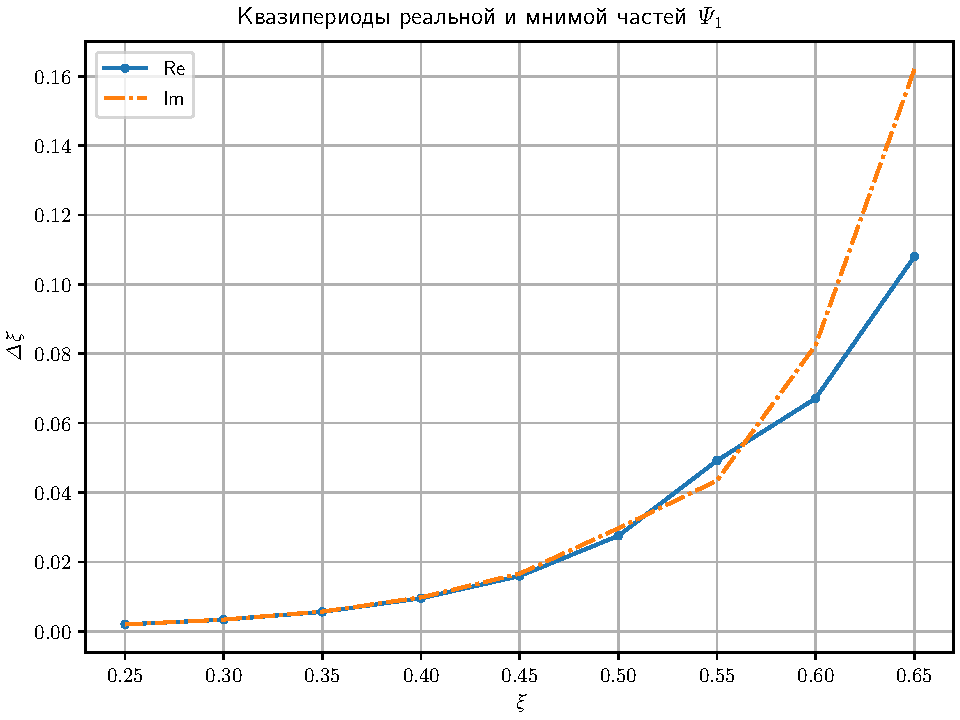
\includegraphics[width=\linewidth]{ri-widths-ru}
\end{frame}

\begin{frame}
	\frametitle{Качественные свойства решения}%
	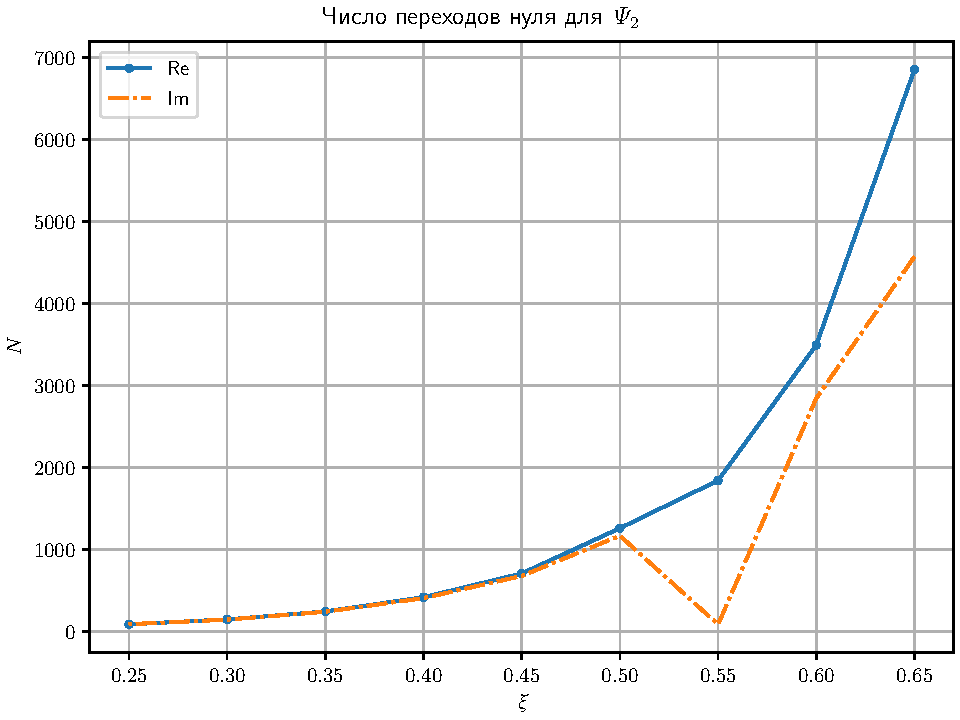
\includegraphics[width=\linewidth]{psi2-trans-ru}
\end{frame}

\begin{frame}
	\frametitle{Качественные свойства решения}%
	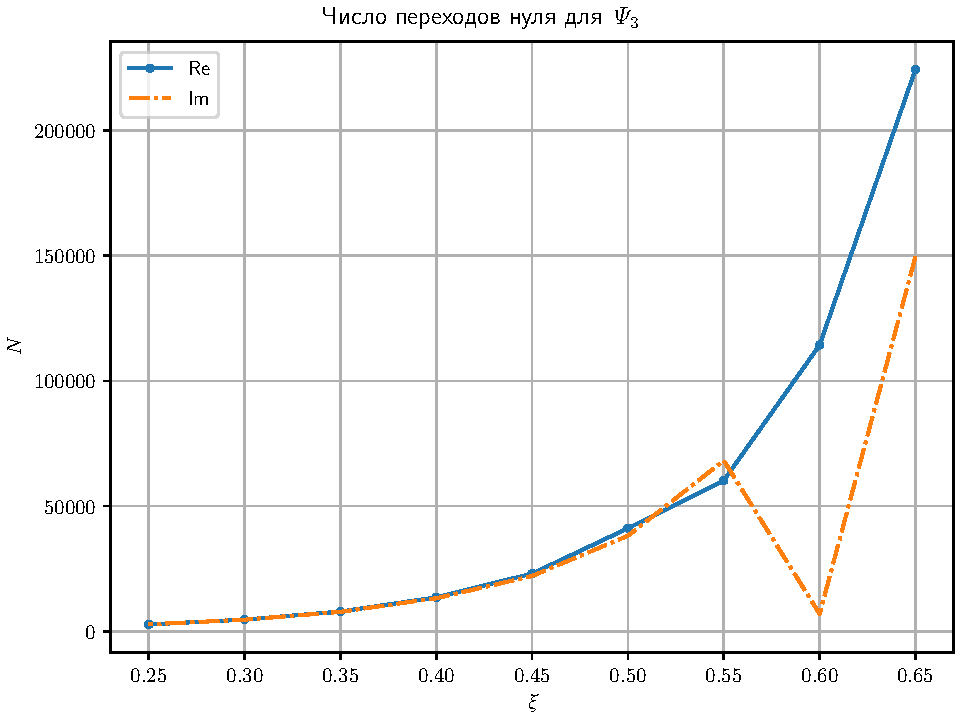
\includegraphics[width=\linewidth]{psi3-trans-ru}
\end{frame}

\begin{frame}
	\frametitle{Качественные свойства решения}%
	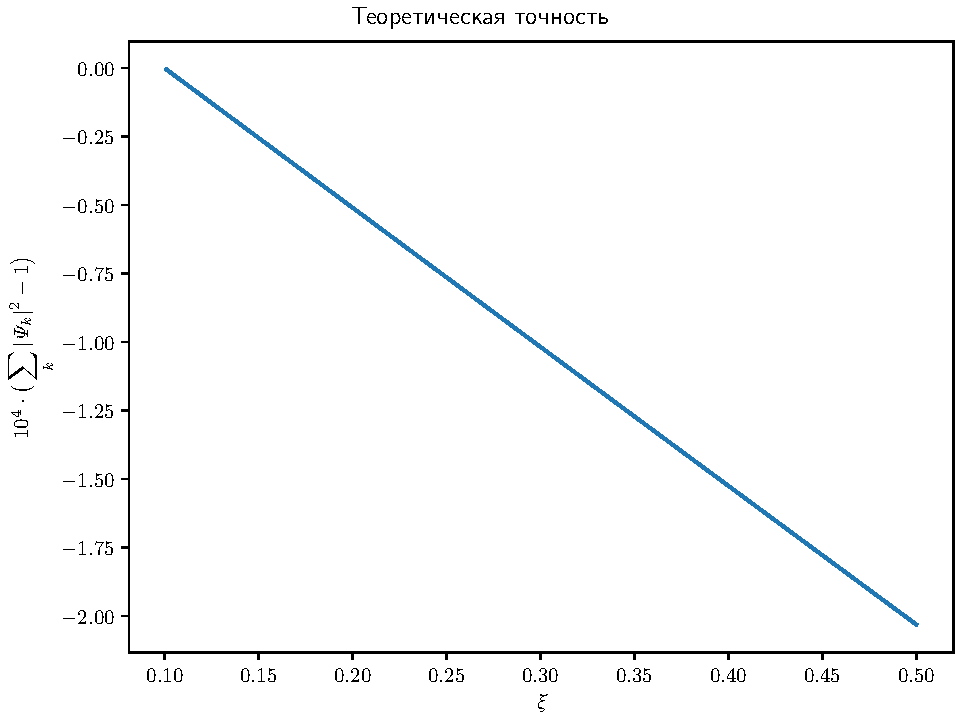
\includegraphics[width=\linewidth]{control-scaled}
\end{frame}

\begin{frame}
	\frametitle{Качественные свойства решения}%
	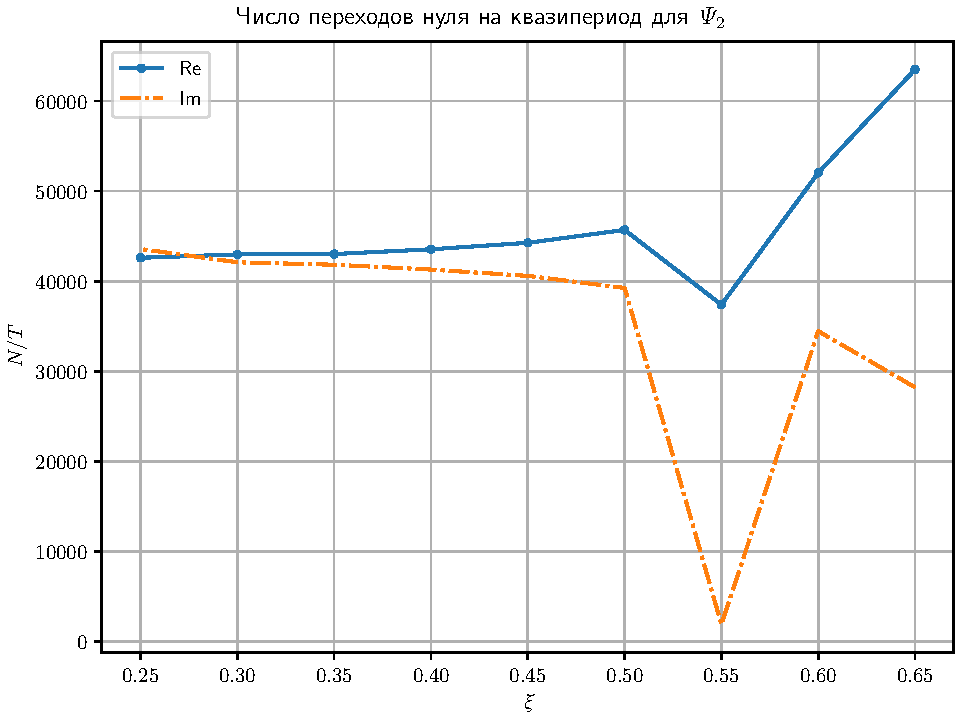
\includegraphics[width=\linewidth]{psi2-rel-trans-ru}
\end{frame}

\begin{frame}
	\frametitle{Качественные свойства решения}%
	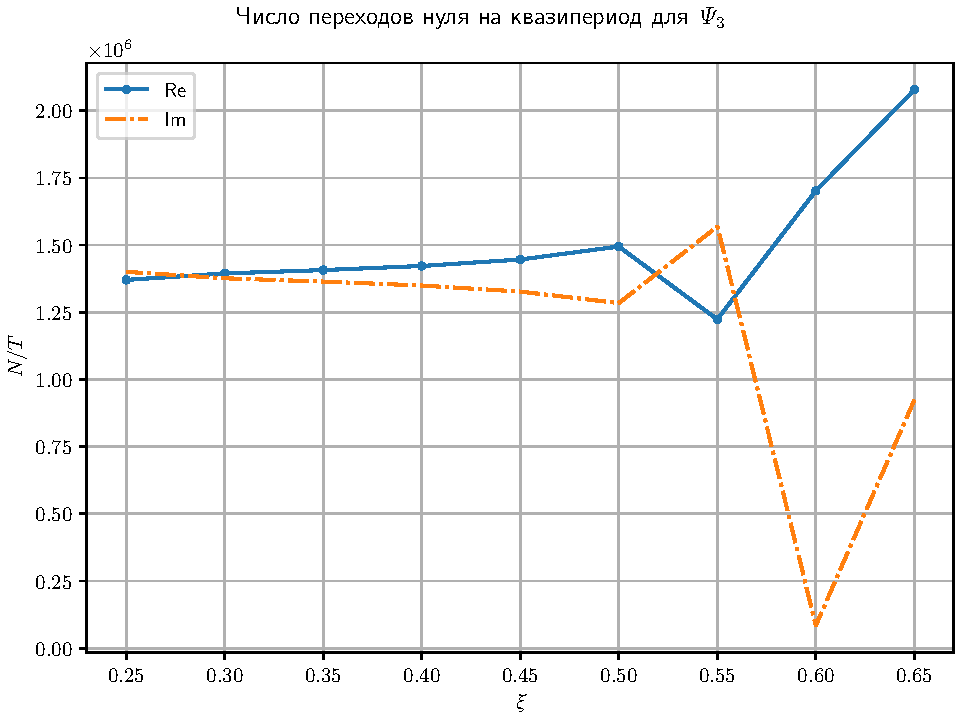
\includegraphics[width=\linewidth]{psi3-rel-trans-ru}
\end{frame}

\begin{frame}
  \frametitle{Заключение}%
  %%%
  В данной работе мы применили встроенные в Mathematica средства численного
  решения дифференциальных уравнений (DOPRI) для выясления качественных
  характеристик полученного решения. 
  \begin{itemize}
  \onslide<2->%
  \item<1-> Мы нашли подходящую характеристику.
  \onslide<3->%
  \item<2->следует внимательно относиться к расчётам с помощью встроенных средств и, по возможности, использовать альтернативные алгоритмы.
  \end{itemize}
\end{frame}

\begin{frame}
  \frametitle{КОНЕЦ}%
  \LARGE%
  \centering%
  \bfseries%
  СПАСИБО ЗА ВНИМАНИЕ%
\end{frame}

\begin{frame}
  \frametitle{Дополнительно}%
  %%%
  \centering%
  ДОПОЛНИТЕЛЬНЫЙ МАТЕРИАЛ
\end{frame}

\end{document}

%%% Local Variables:
%%% mode: latex
%%% fill-column: 80
%%% TeX-master: t
%%% TeX-PDF-mode: t
%%% End:
%%% vim: syn=tex ft=tex tw=80 ts=2 sw=2 et:


% \setbeameroption{show notes on second screen}
\setbeameroption{hide notes}
\mode<presentation>
{
  \usetheme{default}
  %\usecolortheme{default} % dove, beaver
  \usecolortheme{whale}
  %\usefonttheme{serif}
}

\hypersetup{%
  pdfinfo={%
    Title={Защита курсовых работ, ИГУ},%
    Subject={О воспроизводимости результатов численных решений уравнения осцилляции нейтрино в среде},%
    Author={Данеко Илья},%
    Keywords={neutrino oscillation in matter;quality properties}%
  }
}

\title{Качественные свойства решений уравнения осцилляций нейтрино в среде
}%
\author{Данеко И.И.}
\date[ИГУ, 2025]{%
  20 октября 2025\\%
  \vspace*{10ex}%
  \begin{flushright}
    \small
    Научный руководитель: Ломов В.П.\par
  \end{flushright}
  {\vspace*{7ex}
    \footnotesize%
    Иркутск, ФГБОУ ВО ИГУ\par%
  } }

\begin{document}

\begin{frame}
  \titlepage
\end{frame}

\begin{frame}
  \frametitle{Введение}%
  %%%
  % TODO:
  \begin{itemize}
  \item<1->
   Нейтрино — одна из самых необычных частиц в нашем мире.
   
   \item<2->
   Она обладает нулевым зарядом, полуцелым спином и участвует только в слабом
   взаимодействии.
  
  \item<3-> 
  Нейтрино существует как бы в двух видах: флейворные нейтрино и
  массивные. Первые рождаются, тогда как вторые — распространяются.
 
  
  \item<4->% 
   В данной работе мы разбираем качественные
  характеристики численного решения уравнения осцилляции нейтрино в среде.
  \end{itemize}
\end{frame}

\begin{frame}
  \frametitle{Осцилляции нейтрино}%
  %%%
  Три известных состояния флейворных  \({\nu_{\alpha}}(\alpha= e, \mu, \tau)\) являются линейными комбинациями состояний массивных \({\nu_{i}}\) c массами \(m_{i}(i=1,2,3)\), состояния флейворных нейтрино являются суперпозицией состояний массивные нейтрино
  
  \onslide<2->%
  \begin{equation*}\label{eq:1}
  	{\nu_{\alpha}}=\sum_{i}U_{\alpha i}^{*}{\nu_{i}},
  \end{equation*} 
  \(U_{\alpha i}\) являются элементами унитарной матрицы
  смешивания и называемой матрицей Понтекорва–Маки–Накагавы–Сакаты (PMNS).
  
  \onslide<3->%
  Вероятность иметь состояние аромата \(\beta\) в точке r
  \begin{equation*}
  	P_{\alpha\beta}=\sum_{j}|U_{\beta j}|^{2}|A_{j}|^{2}+2\sum_{i>j}Re[U_{\beta i}U_{\beta j}^{*}A_{i}A_{j}^{*}\exp^{-\imath\Delta_{ij}L}].
  \end{equation*}
  Здесь \(\Delta_{ij}=\Delta m_{ij}^2/2E\), где \(E=|p|\), а \(A_{i}\) амплитуда вероятности наличия в точке регестрации
\end{frame}

\begin{frame}
  \frametitle{Осцилляции нейтрино в веществе}%
  %%%
  Уравнение осцилляций в среде
  \begin{equation*}
  	\imath \frac{\partial \Psi}{\partial \xi}=H(\xi)\Psi(\xi).\quad
  \end{equation*}
   \onslide<2->%
  Здесь \({H(\xi)}\) — эрмиртовая матрица
  \begin{equation*}
  	H(\xi)=H_0+\upsilon(\xi)W
  \end{equation*}
   \onslide<3->%
  Матрица \(W\) имеет вид:
  \begin{equation*}
  	W=
  	\begin{pmatrix}
  		c_{13}^{2}c_{12}^{2} & c_{12}s_{12}c_{13}^{2} & c_{12}c_{13}s_{13}\\
  		c_{12}s_{12}c_{13}^{2} & s_{12}^{2}c_{13}^{2} & s_{12}c_{13}s_{13}\\
  		c_{12}s_{13}c_{13} & s_{12}c_{13}s_{13} & s_{13}^{2}
  	\end{pmatrix}.
  \end{equation*}

  \onslide<4->%
  Профиль плотности для солнечной модели
  
  \begin{equation*}
  	\upsilon(\xi)=\gamma exp(-\eta\xi)
  \end{equation*}
  

\end{frame}

\begin{frame}
  \frametitle{Наблюдаемые}%
  %%%
  Вероятность иметь состояние аромата \(\beta\) в точке r
  \begin{equation*}
  	P_{\alpha\beta}=\sum_{j}|U_{\beta j}|^{2}|A_{j}|^{2}+2\sum_{i>j}Re[U_{\beta i}U_{\beta j}^{*}A_{i}A_{j}^{*}\exp(-\imath\Delta_{ij}L)].
  \end{equation*}
  
  \onslide<2->%
  средняя вероятность выживания составляет
  \begin{equation}
  	\langle P_{ee} \rangle=c_{12}^{2}c_{13}^{2}|\Psi_{1}|^{2}+s_{12}^{2}c_{13}^{2}|\Psi_{2}|^{2}+s_{13}^{2}|\Psi_{3}|^{2}.
  \end{equation}
\end{frame}

\begin{frame}
	\frametitle{Качественные свойства решения}%
	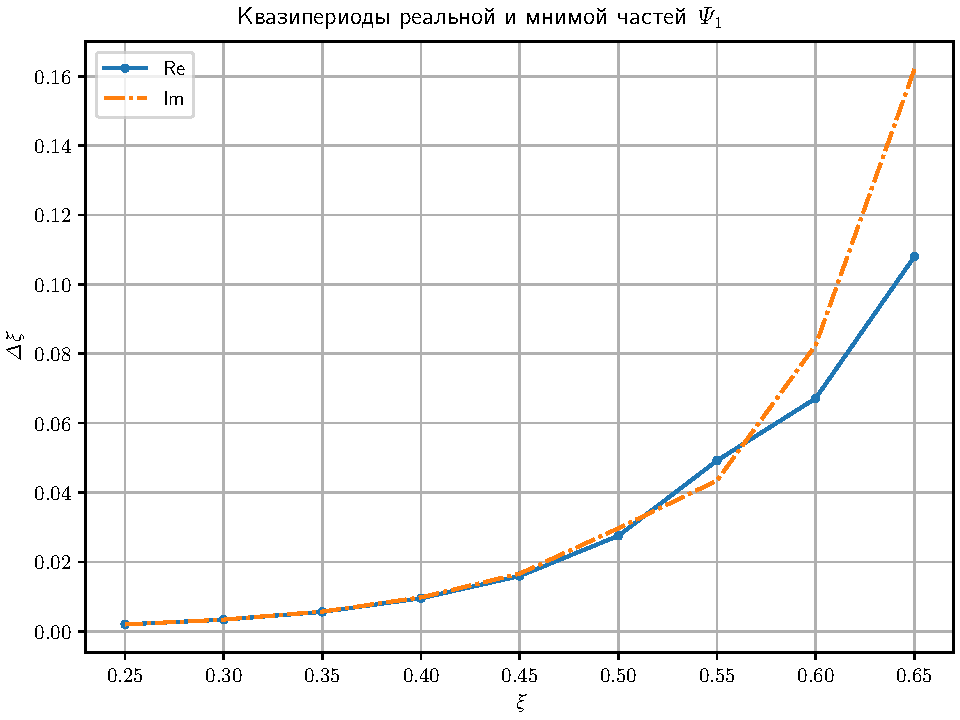
\includegraphics[width=\linewidth]{ri-widths-ru}
\end{frame}

\begin{frame}
	\frametitle{Качественные свойства решения}%
	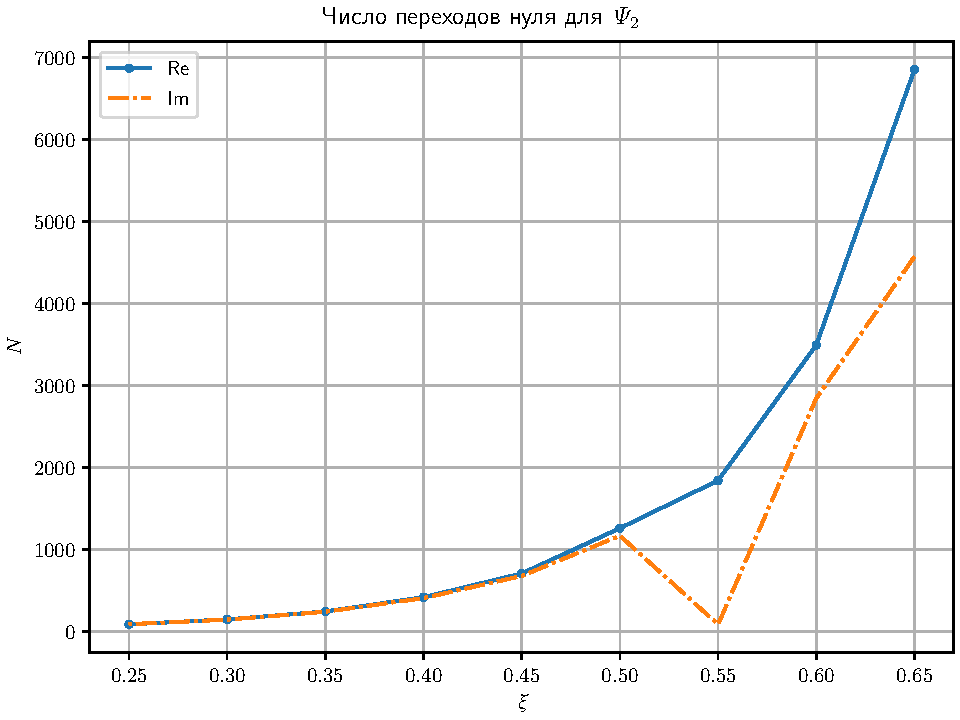
\includegraphics[width=\linewidth]{psi2-trans-ru}
\end{frame}

\begin{frame}
	\frametitle{Качественные свойства решения}%
	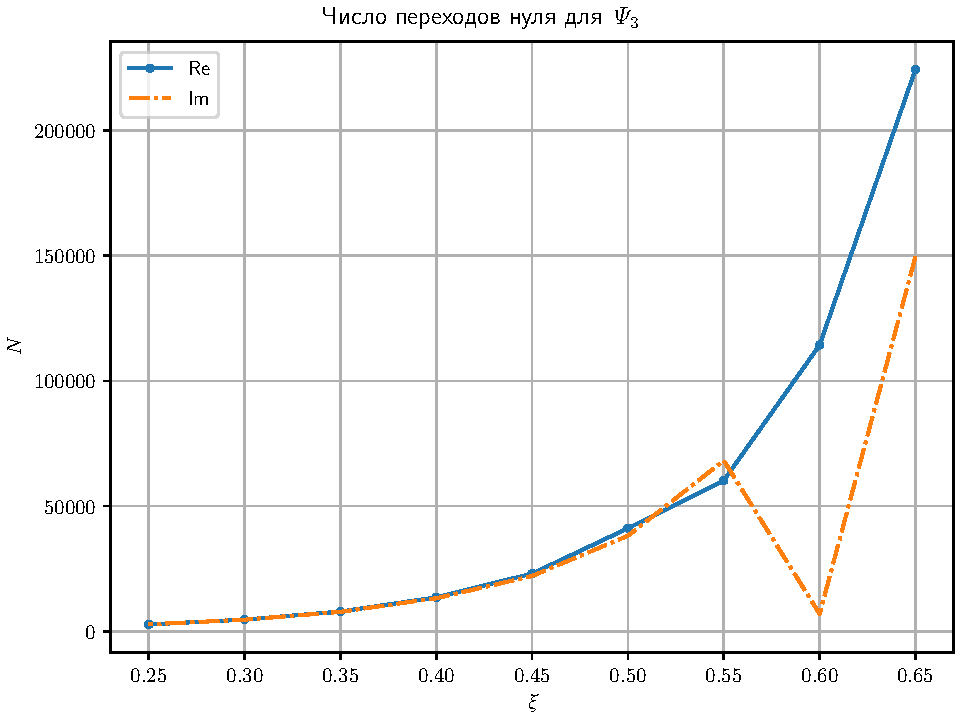
\includegraphics[width=\linewidth]{psi3-trans-ru}
\end{frame}

\begin{frame}
	\frametitle{Качественные свойства решения}%
	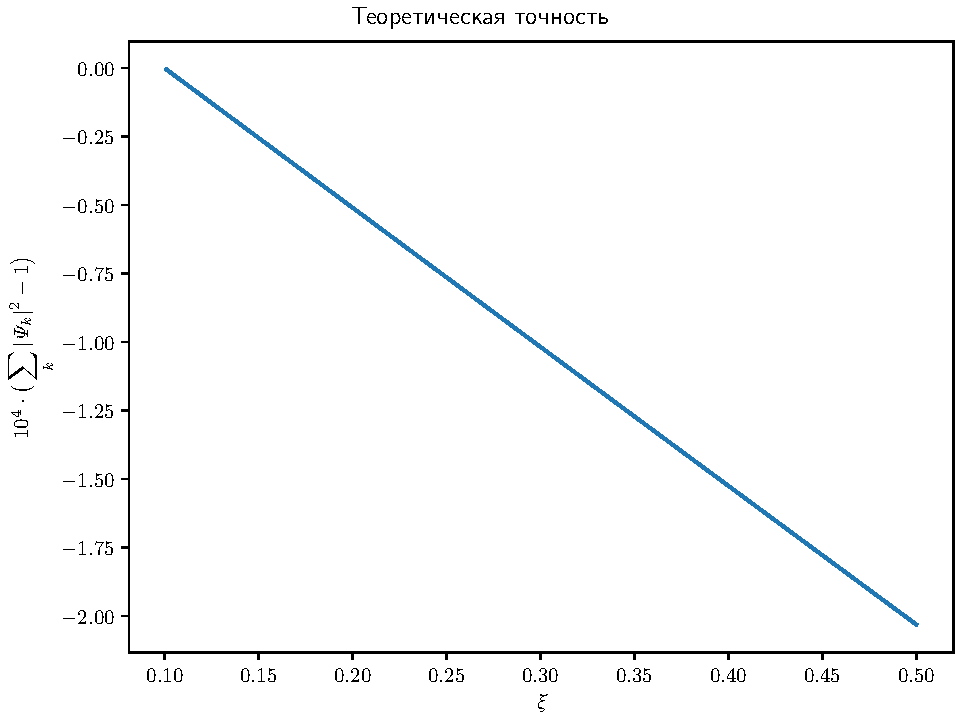
\includegraphics[width=\linewidth]{control-scaled}
\end{frame}

\begin{frame}
	\frametitle{Качественные свойства решения}%
	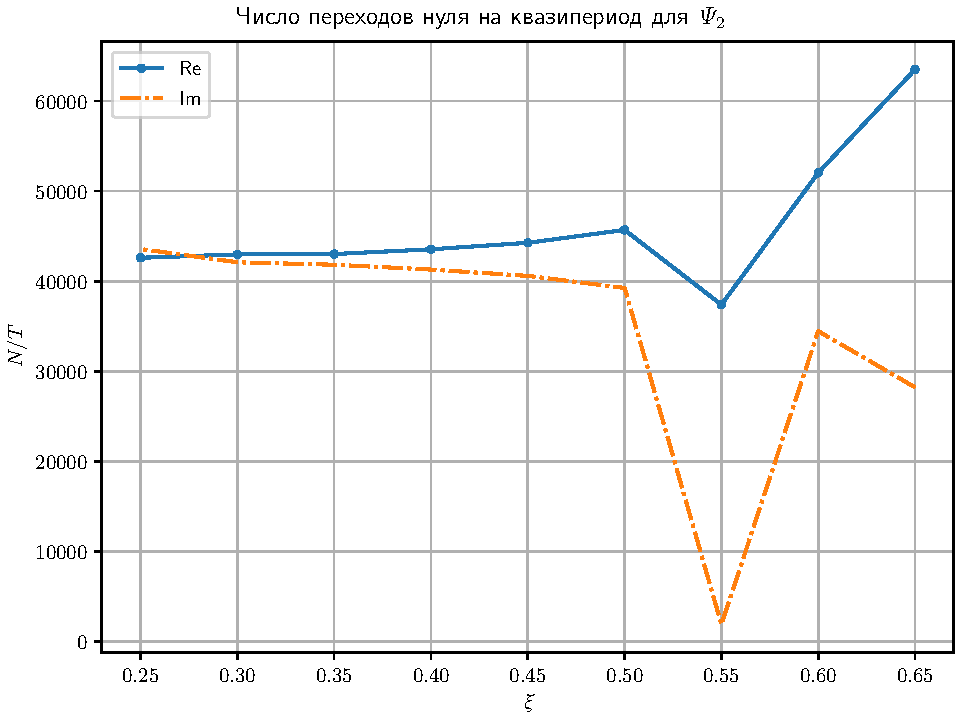
\includegraphics[width=\linewidth]{psi2-rel-trans-ru}
\end{frame}

\begin{frame}
	\frametitle{Качественные свойства решения}%
	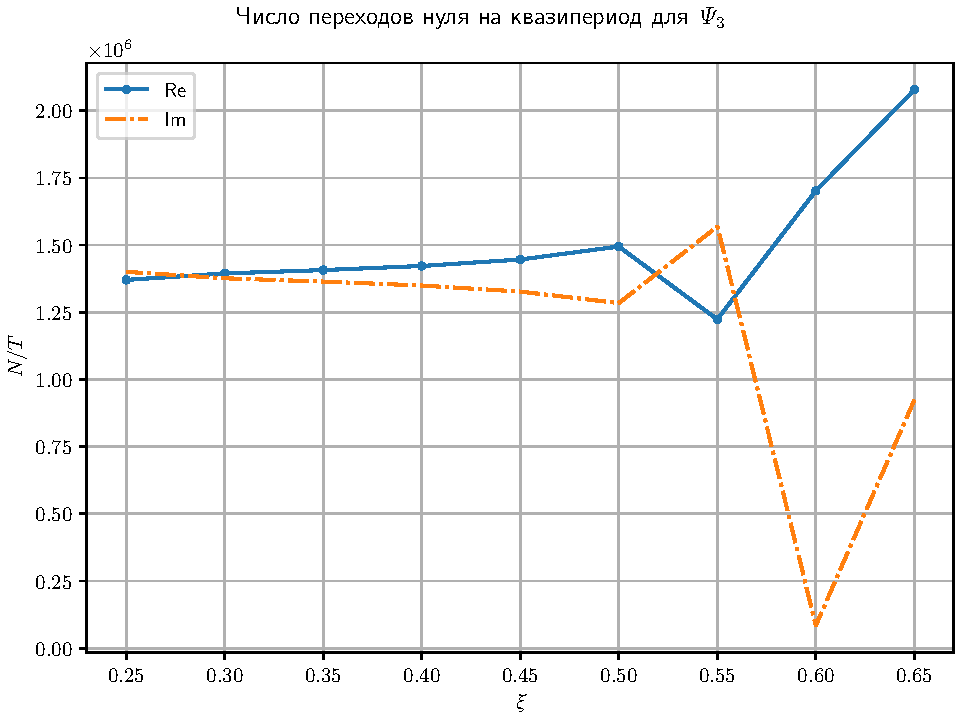
\includegraphics[width=\linewidth]{psi3-rel-trans-ru}
\end{frame}

\begin{frame}
  \frametitle{Заключение}%
  %%%
  В данной работе мы применили встроенные в Mathematica средства численного
  решения дифференциальных уравнений (DOPRI) для выясления качественных
  характеристик полученного решения. 
  \begin{itemize}
  \onslide<2->%
  \item<1-> Мы нашли подходящую характеристику.
  \onslide<3->%
  \item<2->следует внимательно относиться к расчётам с помощью встроенных средств и, по возможности, использовать альтернативные алгоритмы.
  \end{itemize}
\end{frame}

\begin{frame}
  \frametitle{КОНЕЦ}%
  \LARGE%
  \centering%
  \bfseries%
  СПАСИБО ЗА ВНИМАНИЕ%
\end{frame}

\begin{frame}
  \frametitle{Дополнительно}%
  %%%
  \centering%
  ДОПОЛНИТЕЛЬНЫЙ МАТЕРИАЛ
\end{frame}

\end{document}

%%% Local Variables:
%%% mode: latex
%%% fill-column: 80
%%% TeX-master: t
%%% TeX-PDF-mode: t
%%% End:
%%% vim: syn=tex ft=tex tw=80 ts=2 sw=2 et:


% \setbeameroption{show notes on second screen}
\setbeameroption{hide notes}
\mode<presentation>
{
  \usetheme{default}
  %\usecolortheme{default} % dove, beaver
  \usecolortheme{whale}
  %\usefonttheme{serif}
}

\hypersetup{%
  pdfinfo={%
    Title={Защита курсовых работ, ИГУ},%
    Subject={О воспроизводимости результатов численных решений уравнения осцилляции нейтрино в среде},%
    Author={Данеко Илья},%
    Keywords={neutrino oscillation in matter;quality properties}%
  }
}

\title{Качественные свойства решений уравнения осцилляций нейтрино в среде
}%
\author{Данеко И.И.}
\date[ИГУ, 2025]{%
  20 октября 2025\\%
  \vspace*{10ex}%
  \begin{flushright}
    \small
    Научный руководитель: Ломов В.П.\par
  \end{flushright}
  {\vspace*{7ex}
    \footnotesize%
    Иркутск, ФГБОУ ВО ИГУ\par%
  } }

\begin{document}

\begin{frame}
  \titlepage
\end{frame}

\begin{frame}
  \frametitle{Введение}%
  %%%
  % TODO:
  \begin{itemize}
  \item<1->
   Нейтрино — одна из самых необычных частиц в нашем мире.
   
   \item<2->
   Она обладает нулевым зарядом, полуцелым спином и участвует только в слабом
   взаимодействии.
  
  \item<3-> 
  Нейтрино существует как бы в двух видах: флейворные нейтрино и
  массивные. Первые рождаются, тогда как вторые — распространяются.
 
  
  \item<4->% 
   В данной работе мы разбираем качественные
  характеристики численного решения уравнения осцилляции нейтрино в среде.
  \end{itemize}
\end{frame}

\begin{frame}
  \frametitle{Осцилляции нейтрино}%
  %%%
  Три известных состояния флейворных  \({\nu_{\alpha}}(\alpha= e, \mu, \tau)\) являются линейными комбинациями состояний массивных \({\nu_{i}}\) c массами \(m_{i}(i=1,2,3)\), состояния флейворных нейтрино являются суперпозицией состояний массивные нейтрино
  
  \onslide<2->%
  \begin{equation*}\label{eq:1}
  	{\nu_{\alpha}}=\sum_{i}U_{\alpha i}^{*}{\nu_{i}},
  \end{equation*} 
  \(U_{\alpha i}\) являются элементами унитарной матрицы
  смешивания и называемой матрицей Понтекорва–Маки–Накагавы–Сакаты (PMNS).
  
  \onslide<3->%
  Вероятность иметь состояние аромата \(\beta\) в точке r
  \begin{equation*}
  	P_{\alpha\beta}=\sum_{j}|U_{\beta j}|^{2}|A_{j}|^{2}+2\sum_{i>j}Re[U_{\beta i}U_{\beta j}^{*}A_{i}A_{j}^{*}\exp^{-\imath\Delta_{ij}L}].
  \end{equation*}
  Здесь \(\Delta_{ij}=\Delta m_{ij}^2/2E\), где \(E=|p|\), а \(A_{i}\) амплитуда вероятности наличия в точке регестрации
\end{frame}

\begin{frame}
  \frametitle{Осцилляции нейтрино в веществе}%
  %%%
  Уравнение осцилляций в среде
  \begin{equation*}
  	\imath \frac{\partial \Psi}{\partial \xi}=H(\xi)\Psi(\xi).\quad
  \end{equation*}
   \onslide<2->%
  Здесь \({H(\xi)}\) — эрмиртовая матрица
  \begin{equation*}
  	H(\xi)=H_0+\upsilon(\xi)W
  \end{equation*}
   \onslide<3->%
  Матрица \(W\) имеет вид:
  \begin{equation*}
  	W=
  	\begin{pmatrix}
  		c_{13}^{2}c_{12}^{2} & c_{12}s_{12}c_{13}^{2} & c_{12}c_{13}s_{13}\\
  		c_{12}s_{12}c_{13}^{2} & s_{12}^{2}c_{13}^{2} & s_{12}c_{13}s_{13}\\
  		c_{12}s_{13}c_{13} & s_{12}c_{13}s_{13} & s_{13}^{2}
  	\end{pmatrix}.
  \end{equation*}

  \onslide<4->%
  Профиль плотности для солнечной модели
  
  \begin{equation*}
  	\upsilon(\xi)=\gamma exp(-\eta\xi)
  \end{equation*}
  

\end{frame}

\begin{frame}
  \frametitle{Наблюдаемые}%
  %%%
  Вероятность иметь состояние аромата \(\beta\) в точке r
  \begin{equation*}
  	P_{\alpha\beta}=\sum_{j}|U_{\beta j}|^{2}|A_{j}|^{2}+2\sum_{i>j}Re[U_{\beta i}U_{\beta j}^{*}A_{i}A_{j}^{*}\exp(-\imath\Delta_{ij}L)].
  \end{equation*}
  
  \onslide<2->%
  средняя вероятность выживания составляет
  \begin{equation}
  	\langle P_{ee} \rangle=c_{12}^{2}c_{13}^{2}|\Psi_{1}|^{2}+s_{12}^{2}c_{13}^{2}|\Psi_{2}|^{2}+s_{13}^{2}|\Psi_{3}|^{2}.
  \end{equation}
\end{frame}

\begin{frame}
	\frametitle{Качественные свойства решения}%
	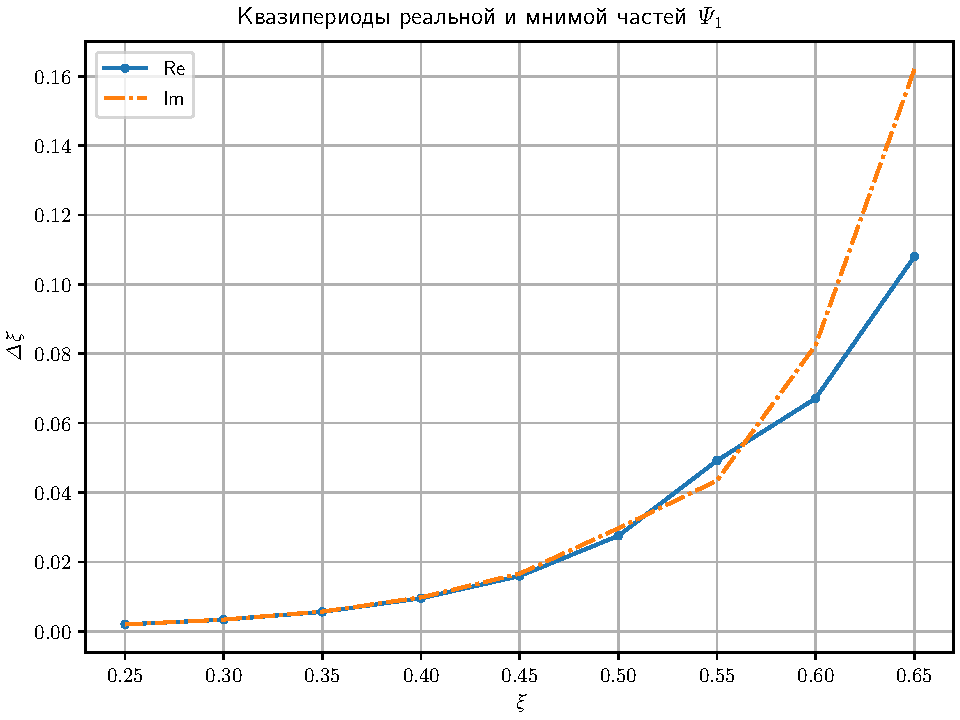
\includegraphics[width=\linewidth]{ri-widths-ru}
\end{frame}

\begin{frame}
	\frametitle{Качественные свойства решения}%
	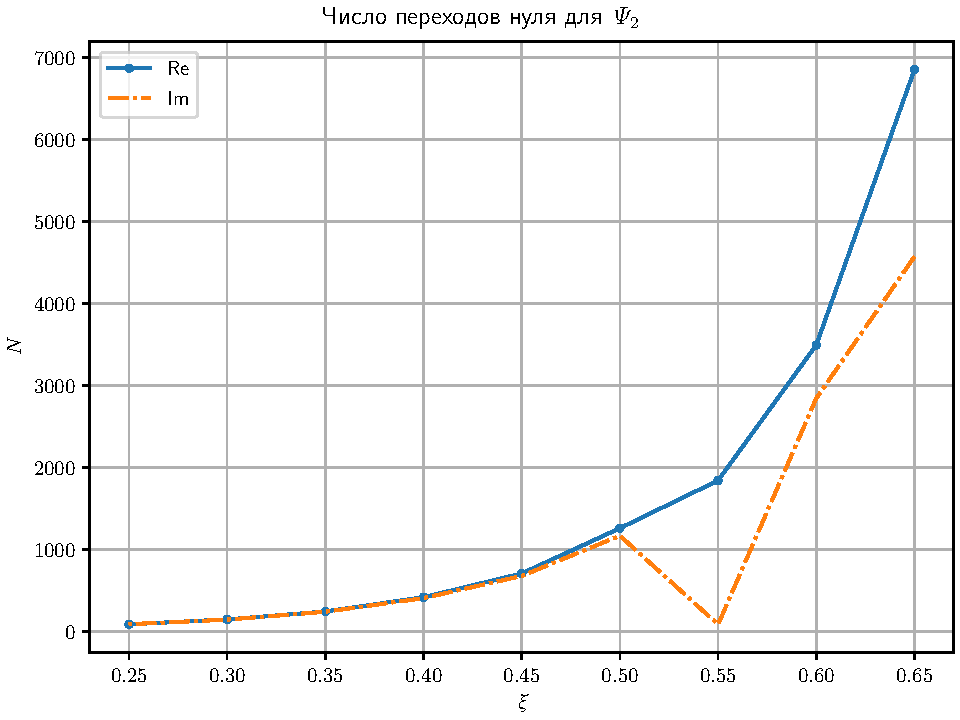
\includegraphics[width=\linewidth]{psi2-trans-ru}
\end{frame}

\begin{frame}
	\frametitle{Качественные свойства решения}%
	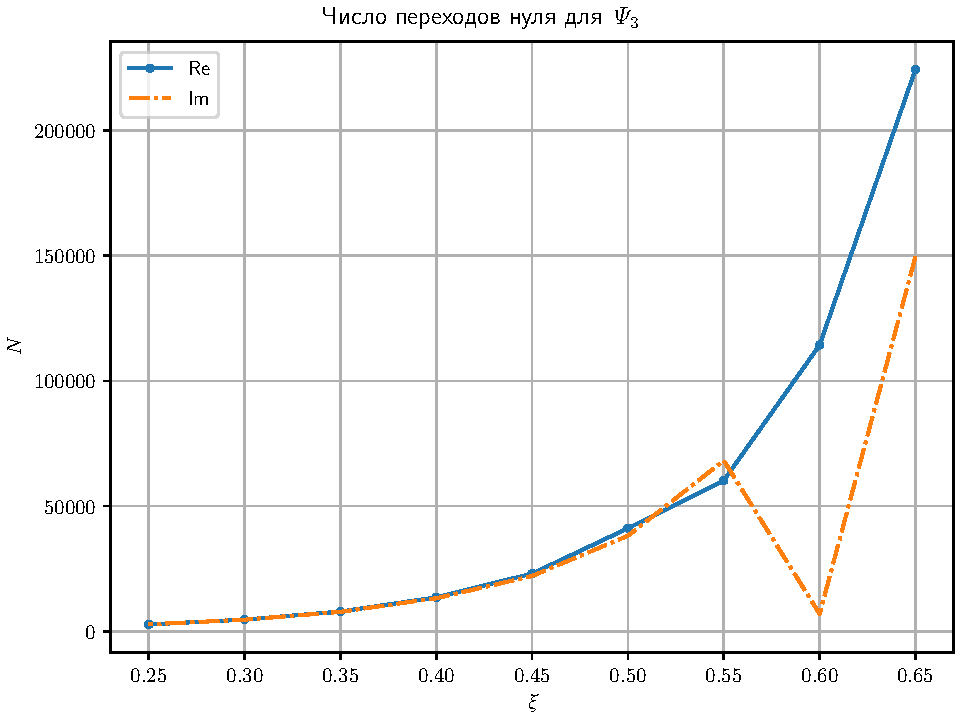
\includegraphics[width=\linewidth]{psi3-trans-ru}
\end{frame}

\begin{frame}
	\frametitle{Качественные свойства решения}%
	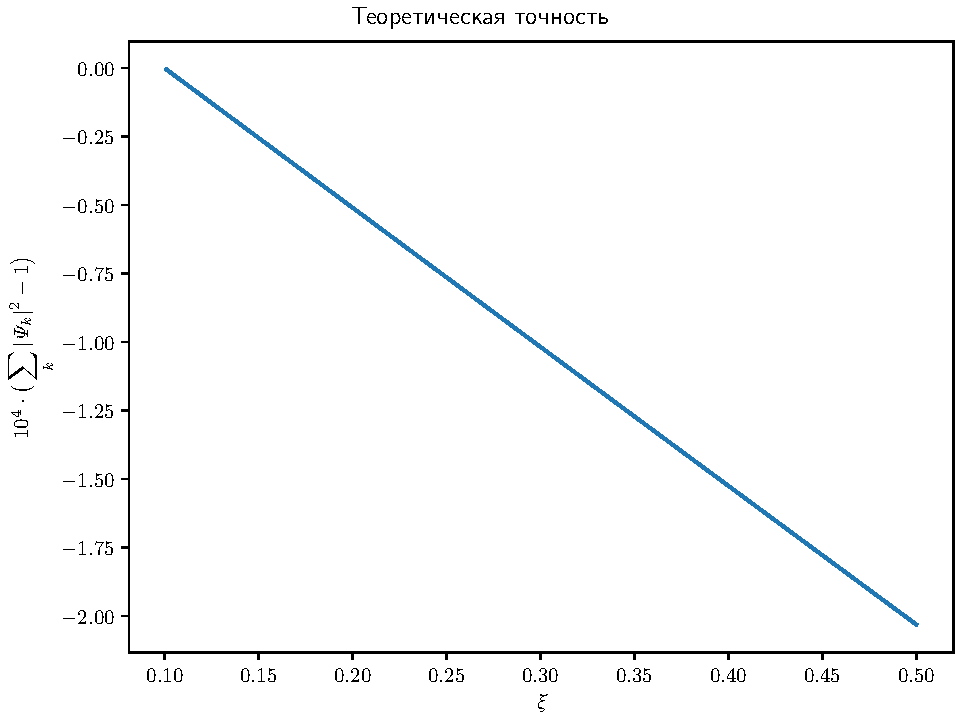
\includegraphics[width=\linewidth]{control-scaled}
\end{frame}

\begin{frame}
	\frametitle{Качественные свойства решения}%
	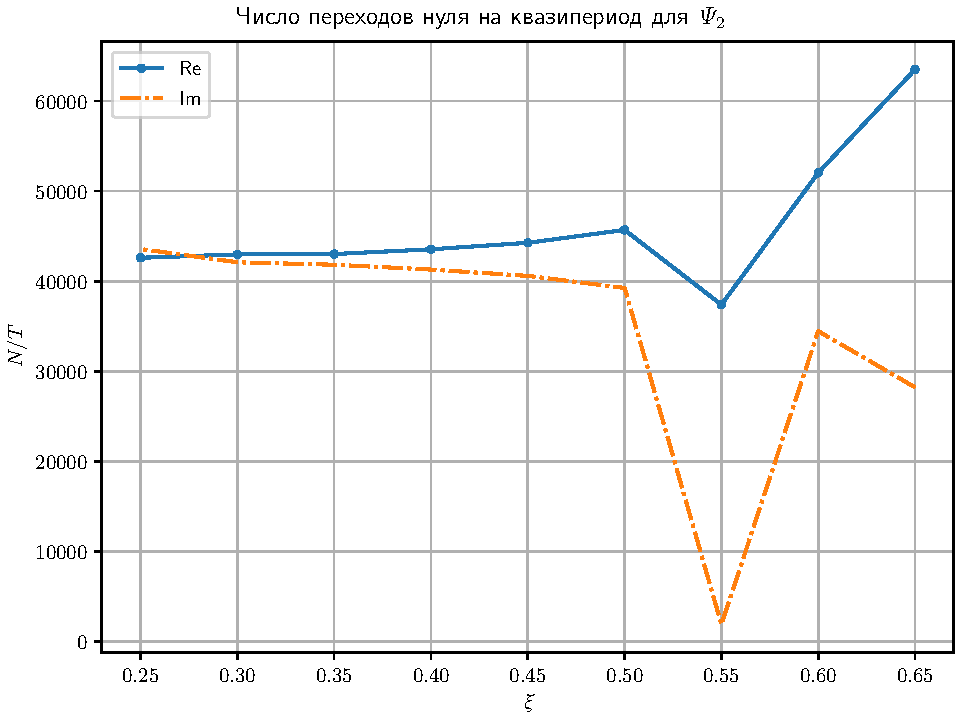
\includegraphics[width=\linewidth]{psi2-rel-trans-ru}
\end{frame}

\begin{frame}
	\frametitle{Качественные свойства решения}%
	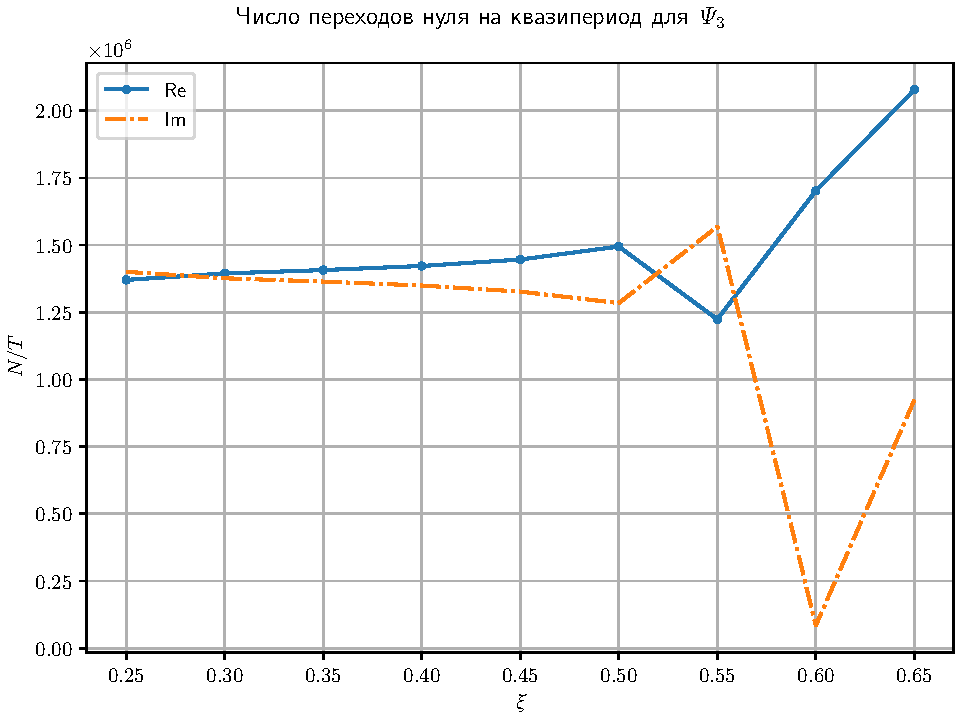
\includegraphics[width=\linewidth]{psi3-rel-trans-ru}
\end{frame}

\begin{frame}
  \frametitle{Заключение}%
  %%%
  В данной работе мы применили встроенные в Mathematica средства численного
  решения дифференциальных уравнений (DOPRI) для выясления качественных
  характеристик полученного решения. 
  \begin{itemize}
  \onslide<2->%
  \item<1-> Мы нашли подходящую характеристику.
  \onslide<3->%
  \item<2->следует внимательно относиться к расчётам с помощью встроенных средств и, по возможности, использовать альтернативные алгоритмы.
  \end{itemize}
\end{frame}

\begin{frame}
  \frametitle{КОНЕЦ}%
  \LARGE%
  \centering%
  \bfseries%
  СПАСИБО ЗА ВНИМАНИЕ%
\end{frame}

\begin{frame}
  \frametitle{Дополнительно}%
  %%%
  \centering%
  ДОПОЛНИТЕЛЬНЫЙ МАТЕРИАЛ
\end{frame}

\end{document}

%%% Local Variables:
%%% mode: latex
%%% fill-column: 80
%%% TeX-master: t
%%% TeX-PDF-mode: t
%%% End:
%%% vim: syn=tex ft=tex tw=80 ts=2 sw=2 et:


% \setbeameroption{show notes on second screen}
\setbeameroption{hide notes}
\mode<presentation>
{
  \usetheme{default}
  %\usecolortheme{default} % dove, beaver
  \usecolortheme{whale}
  %\usefonttheme{serif}
}

\hypersetup{%
  pdfinfo={%
    Title={Защита курсовых работ, ИГУ},%
    Subject={О воспроизводимости результатов численных решений уравнения осцилляции нейтрино в среде},%
    Author={Данеко Илья},%
    Keywords={neutrino oscillation in matter;quality properties}%
  }
}

\title{Качественные свойства решений уравнения осцилляций нейтрино в среде
}%
\author{Данеко И.И.}
\date[ИГУ, 2025]{%
  20 октября 2025\\%
  \vspace*{10ex}%
  \begin{flushright}
    \small
    Научный руководитель: Ломов В.П.\par
  \end{flushright}
  {\vspace*{7ex}
    \footnotesize%
    Иркутск, ФГБОУ ВО ИГУ\par%
  } }

\begin{document}

\begin{frame}
  \titlepage
\end{frame}

\begin{frame}
  \frametitle{Введение}%
  %%%
  % TODO:
  \begin{itemize}
  \item<1->
   Нейтрино — одна из самых необычных частиц в нашем мире.

   \item<2->
   Она обладает нулевым зарядом, полуцелым спином и участвует только в слабом
   взаимодействии.

  \item<3->
  Есть два типа нейтрино: флейворные нейтрино и
  массивные. Первые рождаются, тогда как вторые — распространяются.


  \item<4->%
   В данной работе мы разбираем качественные
  характеристики численного решения уравнения осцилляции нейтрино в среде.
  \end{itemize}
\end{frame}

\begin{frame}
  \frametitle{Осцилляции нейтрино}%
  %%%
  Три флейворных состояния нейтрино \({\nu_{\alpha}}(\alpha= e, \mu, \tau)\)
  являются линейными комбинациями массивных состояний \({\nu_{i}}\) c массами
  \(m_{i}(i=1,2,3)\)
  \onslide<2->%
  \begin{equation*}\label{eq:1}
  	|{\nu_{\alpha}}\rangle=\sum_{i}U_{\alpha i}^{*}|{\nu_{i}}\rangle,
  \end{equation*}
  \(U_{\alpha i}\) — элементы унитарной матрицы
  смешивания, матрица Понтекорво–Маки"=Накагавы"=Сакаты (PMNS).

  \onslide<3->%
  Вероятность найти флейвор \(\beta\) в точке r
  \begin{equation*}
  	P_{\alpha\beta}=\sum_{j}|U_{\beta j}|^{2}|A_{j}|^{2}+
    2\sum_{i>j}\Re[U_{\beta
  	i}U_{\beta j}^{*}A_{i}A_{j}^{*}\exp^{-\imath\Delta_{ij}L}].
  \end{equation*}
  Здесь \(\Delta_{ij}=\Delta m_{ij}^2/2E\), а \(A_{i}\) начальное условие.
\end{frame}

\begin{frame}
  \frametitle{Осцилляции нейтрино в веществе}%
  %%%
  Уравнение осцилляций в среде
  \begin{equation*}
  	\imath \frac{\partial \Psi}{\partial \xi}=H(\xi)\Psi(\xi).\quad
  \end{equation*}
   \onslide<2->%
  Здесь \({H(\xi)}\) — эрмиртовая матрица
  \begin{equation*}
  	H(\xi)=H_0+\upsilon(\xi)W
  \end{equation*}
   \onslide<3->%
  Матрица \(W\) имеет вид:
  \begin{equation*}
  	W=
  	\begin{pmatrix}
  		c_{13}^{2}c_{12}^{2} & c_{12}s_{12}c_{13}^{2} & c_{12}c_{13}s_{13}\\
  		c_{12}s_{12}c_{13}^{2} & s_{12}^{2}c_{13}^{2} & s_{12}c_{13}s_{13}\\
  		c_{12}s_{13}c_{13} & s_{12}c_{13}s_{13} & s_{13}^{2}
  	\end{pmatrix}.
  \end{equation*}

  \onslide<4->%
  Профиль плотности для солнечной модели

  \begin{equation*}
  	\upsilon(\xi)=\gamma \exp^{-\eta\xi}
  \end{equation*}
\end{frame}

\begin{frame}
  \frametitle{Наблюдаемые}%
  %%%
  Вероятность иметь состояние аромата \(\beta\) в точке r
  \begin{equation*}
  	P_{\alpha\beta}=\sum_{j}|U_{\beta j}|^{2}|A_{j}|^{2}+2\sum_{i>j}\Re[U_{\beta
  	i}U_{\beta j}^{*}A_{i}A_{j}^{*}\exp(-\imath\Delta_{ij}L)].
  \end{equation*}

  \onslide<2->%
  Усреднённая вероятность выживания составляет
  \begin{equation*}
  	\langle P_{ee}\rangle
    =c_{12}^{2}c_{13}^{2}|\Psi_{1}|^{2}+s_{12}^{2}c_{13}^{2}|\Psi_{2}|^{2}+s_{13}^{2}|\Psi_{3}|^{2}.
  \end{equation*}
\end{frame}

\begin{frame}
	\frametitle{Качественные свойства решения}%
	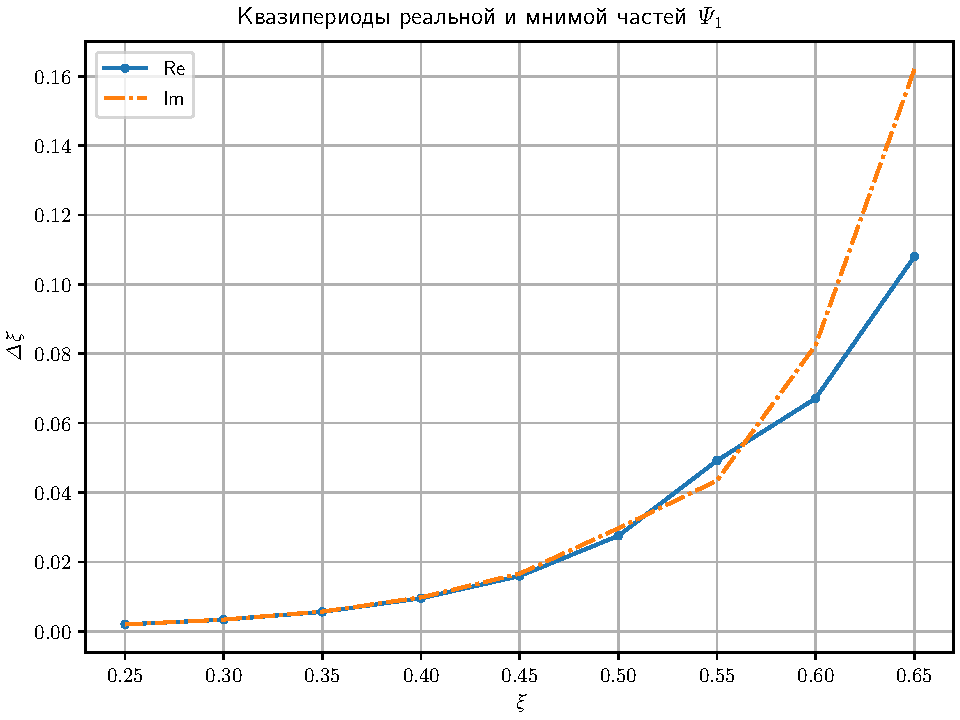
\includegraphics[width=\linewidth]{ri-widths-ru}
\end{frame}

\begin{frame}
	\frametitle{Качественные свойства решения}%
	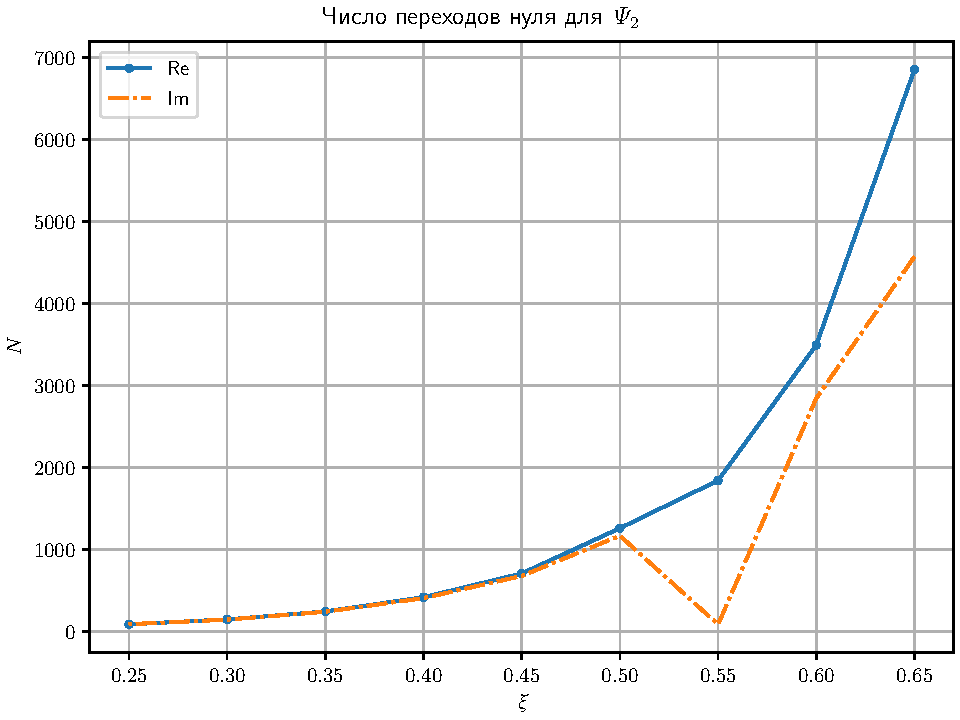
\includegraphics[width=\linewidth]{psi2-trans-ru}
\end{frame}

\begin{frame}
	\frametitle{Качественные свойства решения}%
	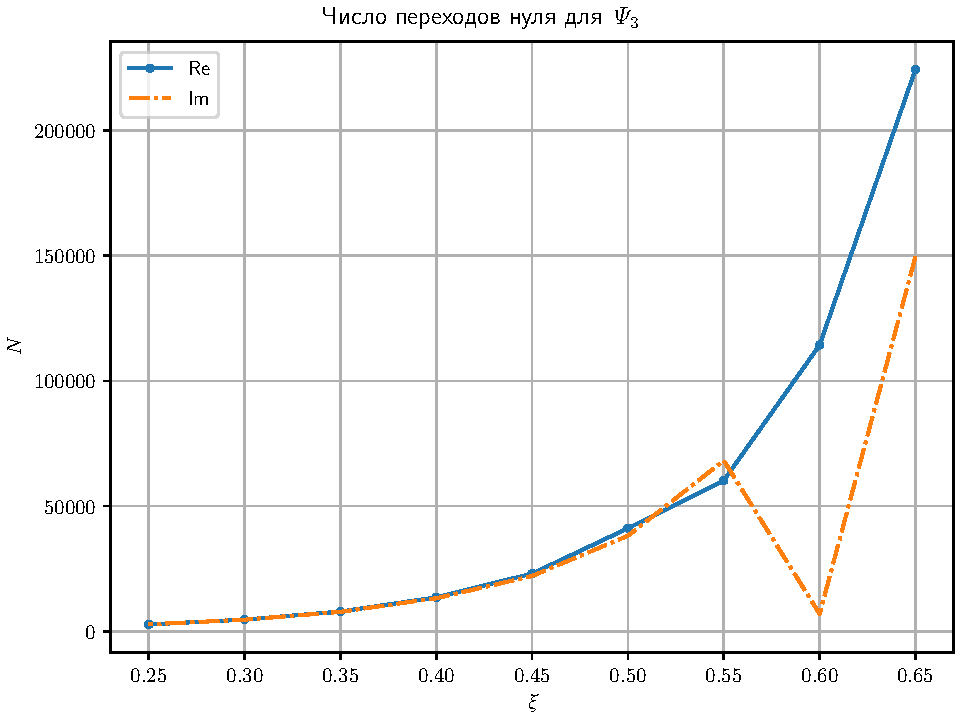
\includegraphics[width=\linewidth]{psi3-trans-ru}
\end{frame}

\begin{frame}
	\frametitle{Качественные свойства решения}%
	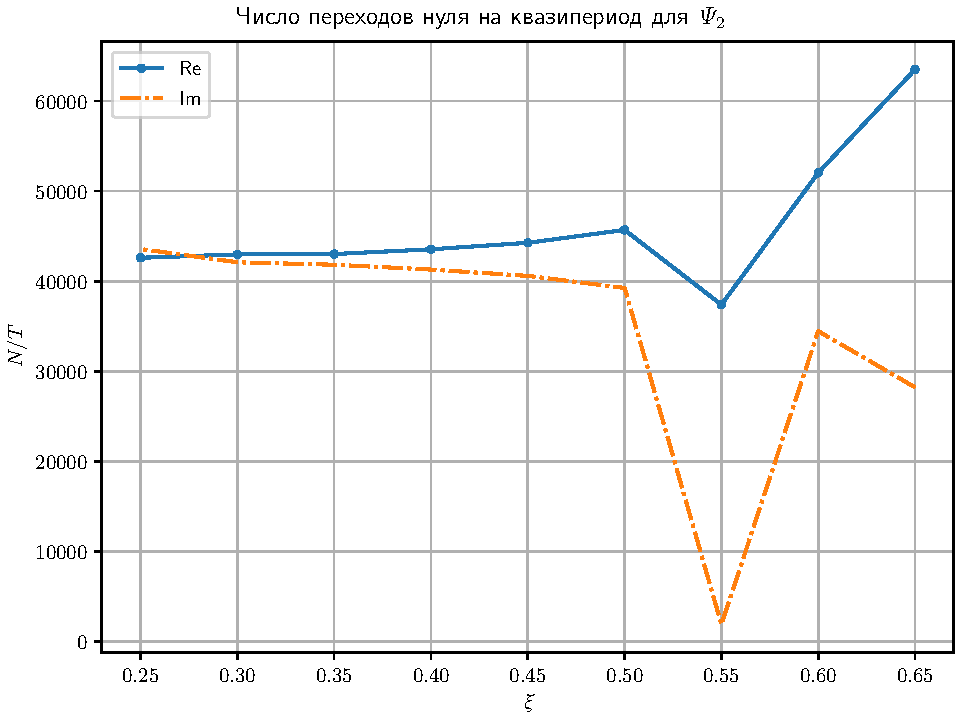
\includegraphics[width=\linewidth]{psi2-rel-trans-ru}
\end{frame}

\begin{frame}
	\frametitle{Качественные свойства решения}%
	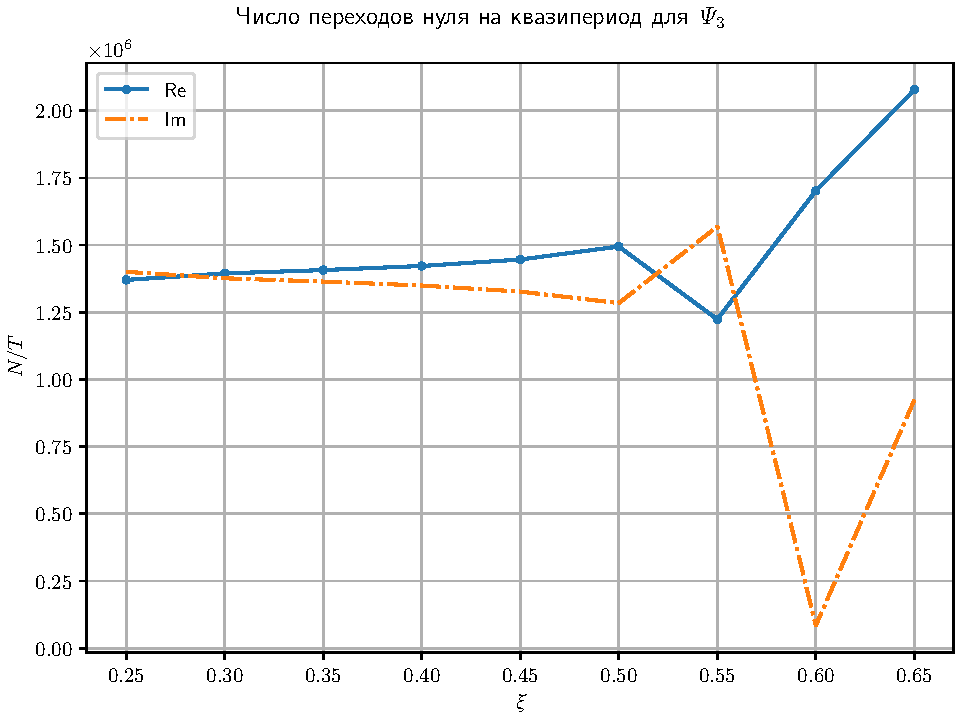
\includegraphics[width=\linewidth]{psi3-rel-trans-ru}
\end{frame}

\begin{frame}
  \frametitle{Качественные свойства решения}%
  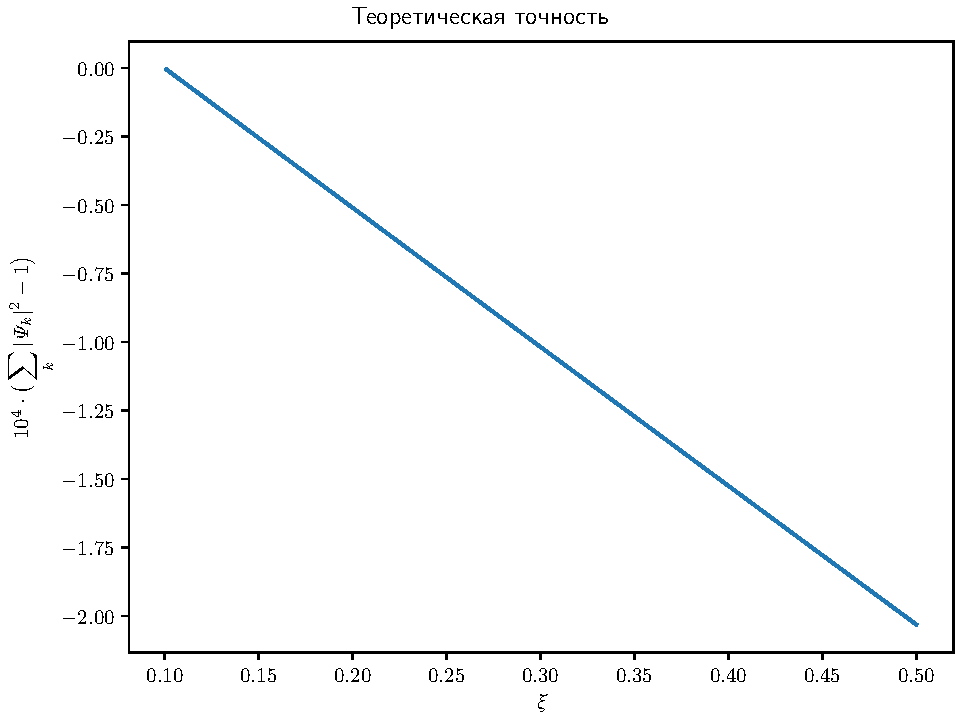
\includegraphics[width=\linewidth]{control-scaled}
\end{frame}

\begin{frame}
  \frametitle{Заключение}%
  %%%
  В данной работе мы применили встроенные в Mathematica средства численного
  решения дифференциальных уравнений (DOPRI) для выясления качественных
  характеристик полученного решения.
  \begin{itemize}
  \onslide<2->%
  \item<1-> Мы нашли подходящую характеристику.
  \onslide<3->%
  \item<2->Следует внимательно относиться к расчётам с помощью встроенных средств
  и, по возможности, использовать альтернативные алгоритмы.
  \end{itemize}
\end{frame}

\begin{frame}
  \frametitle{КОНЕЦ}%
  \LARGE%
  \centering%
  \bfseries%
  СПАСИБО ЗА ВНИМАНИЕ%
\end{frame}

\end{document}

%%% Local Variables:
%%% mode: latex
%%% fill-column: 80
%%% TeX-master: t
%%% TeX-PDF-mode: t
%%% End:
%%% vim: syn=tex ft=tex tw=80 ts=2 sw=2 et:
